\documentclass[20pt]{article}
\usepackage[utf8]{inputenc}

\title{\textbf{Week 4:} 
\underline{Self Learning Topic Introduction}}
\usepackage{graphicx}

\author{Isaac Kim}
\date{March 2022}

\begin{document}
\maketitle 

\section{What is PyGame?}
Pygame is a cross-platform set of Python modules designed for writing video games. It includes computer graphics and sound libraries designed to be used with the Python programming language.

\section{PyGame Logo}
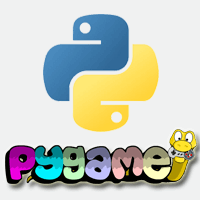
\includegraphics{pygame_logo.png}

\section{Why learn PyGame?}
I think Pygame is a great tool for beginners like myself to get comfortable with more advanced 
features of a programming language and usage of many modules/tools of python. Meanwhile, it also 
introduces the process of game development, an area I'm particularly interested in the field of computer science.

\section{Projects created in PyGame}

\includegraphics{pygameEx1.jpg}
\\
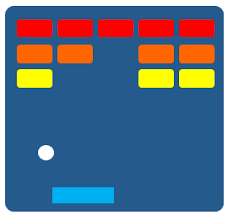
\includegraphics{PygameEx2.png}
\end{document}